\section{Introduction}
% memo
% worldbank website: http://www.worldbank.org/en/about/what-we-do
%For any serious human activity, there is the natural question: what difference does it make? 
%If one leaves the realm of scientific lab experiments, the challenge is that the ?ground truth? for a causal effect is not
%observed for any individual unit: we observe the unit with the treatment, or without the treatment, but not both at the same time,
%
%For a large scale, worldwide operation like the world bank, this question is particularly challenging to answer. 
%The world bank's overarching goal is in economic development;  it formulates this as to "end extreme poverty by decreasing the percentage of people living on less than \$1.90 a day to no more than 3\%"  and to "promote shared prosperity by fostering the income growth of the bottom 40\% for every country" \cite{worldbankwebsite}.
%Each individual project that it funds extends over time, so what is an appropriate measure of difference over time?
%Each individual project is located in space, so what is an appropriate measure of difference in space?
%
%Some notes
%\begin{itemize}
%\item general problem in development: project has a time, space, and economic dimension, 
%\item how to measure success
%\item how to measure what's going on
%\item how to measure impact (and when), how to infer causality
%\item problem present in particular in aid projects for third world
%\item describe data
%\item formulate research question that is addressed 
%\item countries that have bad causal or good effects across different project starting years for the 5 continents
%\item figure show aid project in the world map
%
%\item main area or countries that have good or bad effects
%\end{itemize}

\begin{figure}
	\centering
	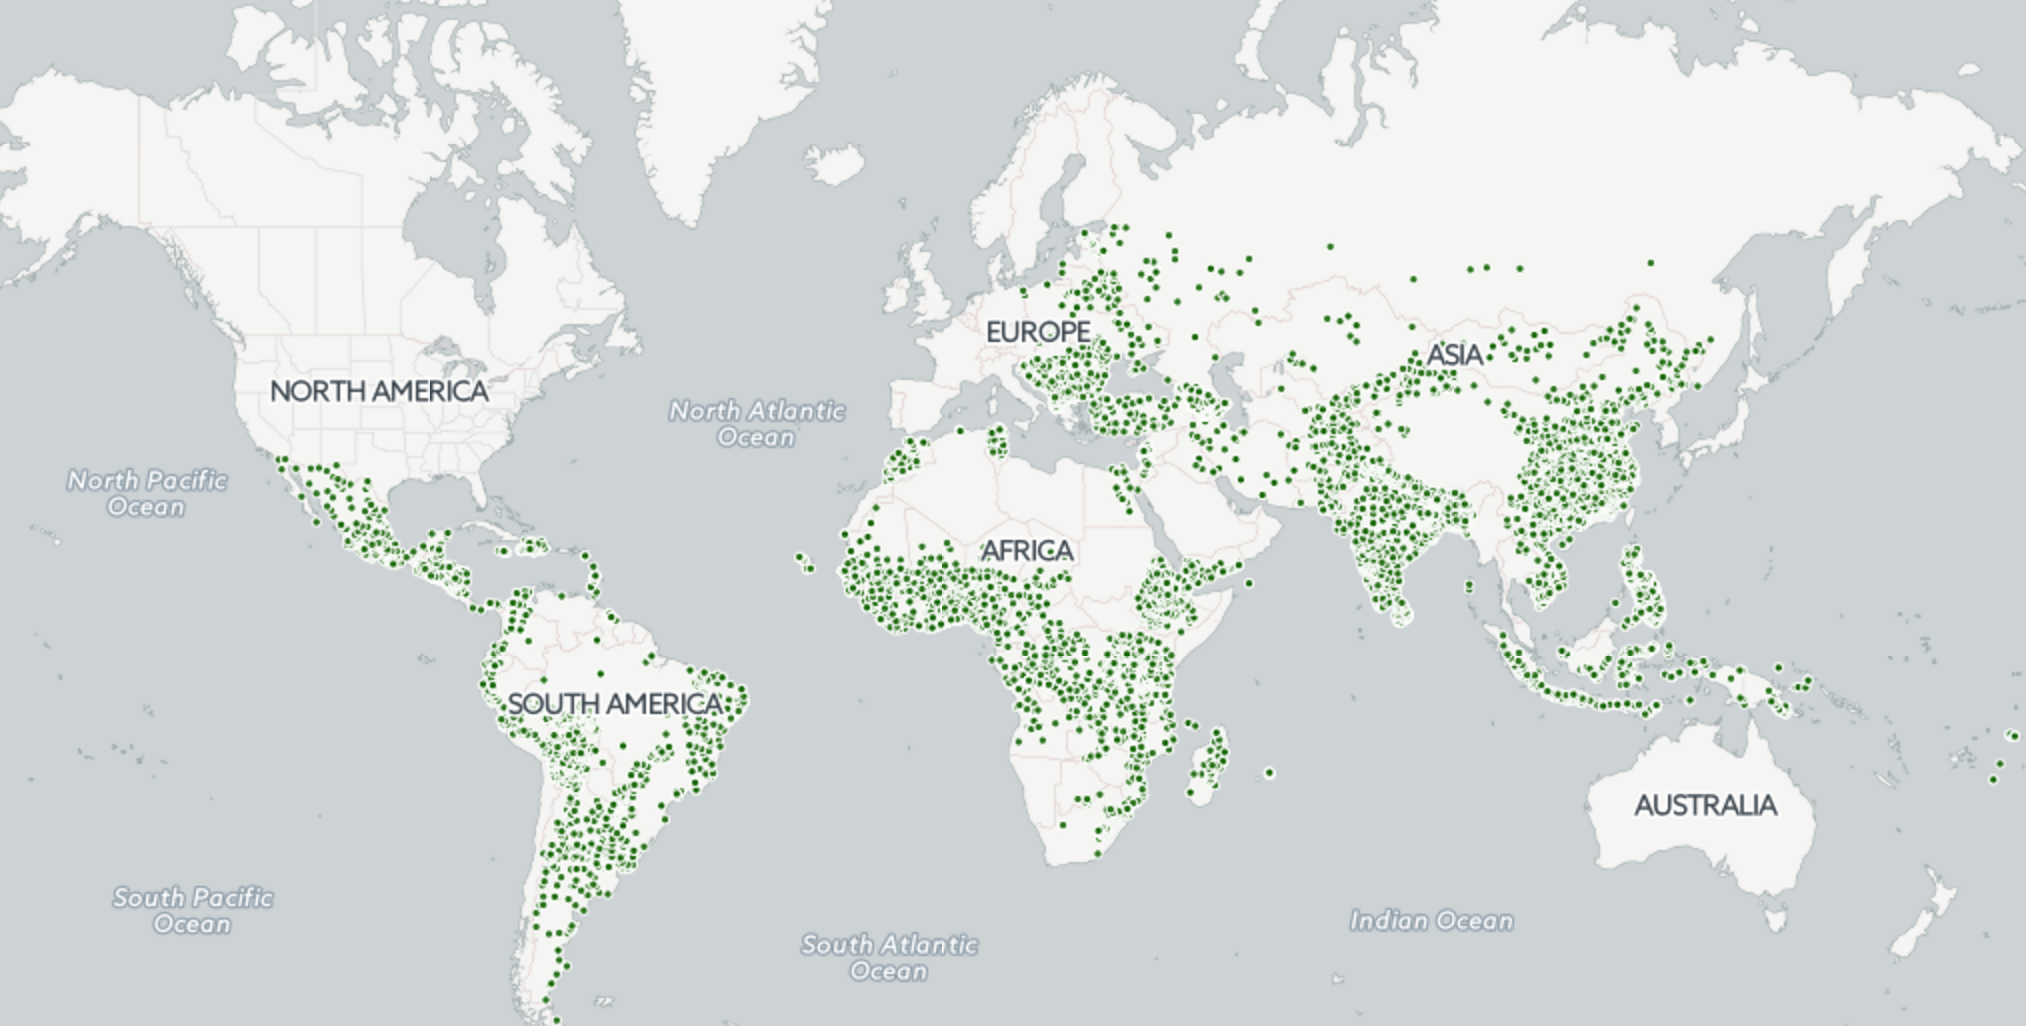
\includegraphics[width=\textwidth]{figs/wbprojects.png}
	\caption{world bank projects} \label{fig:wbprojects}
\end{figure}

For any serious human activity, there is the natural question: what difference does it make? 
Identifying and quantifying causal effects from data is one of the most interesting  research problem across many disciplines. 
For example, this arises in measuring the effectiveness of a drug in medical studies, in measuring the impact of changes in an e-commerce website design on customers, in evaluating the effectiveness of public policies. In our case, the world bank is interested in measuring the impact of aid projects it funded and supported all over the world over 30 years. 

The world bank's overarching goal is in economic development;  it formulates this as to "end extreme poverty by decreasing the percentage of people living on less than \$1.90 a day to no more than 3\%"  and to "promote shared prosperity by fostering the income growth of the bottom 40\% for every country" \cite{worldbankwebsite}. At an abstract level, the world bank provides funding for aid projects and can rely on a metric of choice to measure differences before a project begins and after a project ends. 
At the level of an individual project, we face the general crux of all observational studies, i.e., we can not observe the exact same geographic, environmental, social, economic, and historical setting with or without the project. So for measuring a difference, one has to rely on making meaningful comparisons between locations that are sufficiently similar. In addition to that, the world bank's operation is large scale with a large number of projects and worldwide, which creates a huge variability in the specific kind of project, the project's size, location, socio-economic, environmental, and historical setting. Figure \ref{fig:wbprojects} shows the locations of a set of world bank projects with 1168 projects in 16415 locations  that were performed between 2001 and 2012 on a global map.

The research questions, we investigate in this paper are:
\begin{itemize}
\item Can we estimate the impact of a project?
\item Can we identify subsets of entities in our data set that are meaningful to compare?
\item Can we identify attributes that are indicative of projects that show a positive (or negative) impact?
\end{itemize}

To do so, we enhance a given data set of world bank projects with additional information about the geographic, environmental, and economic 
characteristics over a number of years and rely on state-of-the-art techniques to estimate heterogenous causal effects. 
In our case, it is not interesting to estimate the overall average effect of all aid projects, but to identify subsets of projects by attributes and estimate average effects for individual subsets.
%Instead of investigate the causal effects for the whole population, in this paper, we are interested in estimating heterogeneous causal effects for subpopulations by features or covariates. We can estimate heterogeneity by covariates on causal effects and then conducting inference for a distinct unit.\\
%To avoid getting extreme treatment effects which lead to a spurious heterogeneous result, in disciplines such as clinical trial, they use pre-planed subgroup to analyze, for economic, they have pre-analysis plans for randomized experiments. With a data driven approach, the advantage is to discover some other causal effects instead of only the pre-planed subgroups.\\
To estimate heterogenous causal effects, there are several candidates, such as classification and regression trees  \cite{Breiman:2001:RF:570181.570182}, random forests \cite{breiman1984classification}, LASSO \cite{Tibshirani94regressionshrinkage}, and support vector machines (SVM) \cite{Vapnik1998}. 
%In this paper, we use the regression tree, the other methods such as random forest is also good candidate, but we focus on the regression tree in this paper.\\
In this paper, we follow the work of Athey and Imbens \cite{1504.01132} who demonstrated how regression trees and in conclusion also random forests can be adjusted to estimate heterogenous causal effects. It is based on the Rubin Causal Model or potential outcome framework where causal effects are comparisons between observed outcomes and counterfactual outcomes one would have observed under the absence of an aid project \cite{Imbens:2015:CIS:2764565}. Regression trees and random forests in traditional machine learning rely on training with data with known outcomes. Athey and Imbens showed that one can estimate the conditional average treatment effect on a  subset with regressions trees after an appropriate data transformation using propensity scores. This leads to the notion of transformed-outcome trees and causal trees that we use for our analysis. 

The rest of the paper is structured as follows. In Section 2, we recall the basic methodology for the calculation of transformed-outcome trees, causal trees, and random forests.  Section 3 introduces the data set, its characteristics, preprocessing steps and the calculation of propensity scores. In Section 4, we present the outcome of the analysis. We conclude in Section 5.
%In tradition, we can use decision trees to do prediction using the trained data or labeled data. We can build the regression tree to predicting the causal effects with the features as nodes in the tree. However, for the causal inference, the challenge is we do not have such data,in rubin causal model \cite{Imbens:2015:CIS:2764565}, we can only have the treated data or untreated data, but not both at the same time, hence we do not know the ground truth for prediction. We can't follow the traditional supervised machine learning method that we contract the tree with the trained the data and then use the the test data to do prediction based on the constructed tree. Follow the work of Athey and Imbens \cite{1504.01132}, we use causal tree to do heterogeneous causal effects estimation. However, in practice,for example in our case the world bank data set, within a node, there maybe only treated or untreated data, we will discuss in the paper how to explain such data and other issues \\
%\begin{itemize}
%\item first analysis on heterogeneous causal effect of world bank aid projects using machine learning method
%\item 
%
%\end{itemize}
